% !TEX spellcheck = en_US

\documentclass[conference]{IEEEtran}
\usepackage{cite}
\usepackage{amsmath,amssymb,amsfonts}
\usepackage{algorithmic}
\usepackage{graphicx}
\usepackage{textcomp}
\usepackage{xcolor}
% add hyperlinks, delete all .aux files if adding hyperref after previous build
\usepackage{hyperref}
% support for unicode charcters like "é" and "ñ"
\usepackage[T1]{fontenc}
% Provides generic commands \degree, \celsius, \perthousand, \micro and \ohm
\usepackage{gensymb}
% splits a section into multiple columns
\usepackage{multicol}
\def\BibTeX{{\rm B\kern-.05em{\sc i\kern-.025em b}\kern-.08em
    T\kern-.1667em\lower.7ex\hbox{E}\kern-.125emX}}
\begin{document}

\title{Comparison of Predicted PV System Performance with SURFRAD versus TMY}

\author{\IEEEauthorblockN{Mark A. Mikofski and Rounak Kharait}
	\IEEEauthorblockA{DNV, Oakland, CA, 9612, USA }}

\maketitle

\begin{abstract}
Solar resource is important for predicting PV system performance. Historical Typical Meteorological Years (TMY) from 1960-1990 and 1990-2005 are commonly used in the United States, but recently there have been concerns by stakeholders whether these data-sets may lead to over-predictions. Therefore we simulated performance of a fictional PV system with over 20-years of accurate ground based surface radiation (SURFRAD) measurements at 7 locations and compared the median year performance with simulations using TMY data. We found that the NREL Physical Solar Model V3 (PSM3) performance predictions were greater than all SURFRAD years at 5 sites, TMY2 predictions were greater than 70-90\% of SURFRAD years at 5 sites, and TMY3 predictions were closest to the median.
\end{abstract}

\begin{IEEEkeywords}
SURFRAD, TMY, irradiance, PV, performance, prediction
\end{IEEEkeywords}

\section{Introduction}
Investors require accurate predictions of PV system performance to quantify and manage their risks. However, there is growing concern about under-performing PV systems \cite{Matsui2020}. Predictions commonly use TMY data-sets developed from historical data. There are many sources of TMY data sets, but we focused on three publicly available TMY data-sets from the National Renewable Energy Laboratory (NREL), and compared them with accurate, ground-based, high-frequency SURFRAD data at 7 sites from 1995 until present day \cite{Augustine2000} by simulating a fictional PV system. Our goal was to determine if the predictions with TMY data would yield the same median performance we simulated with the SURFRAD data, but we discovered the TMY over-predicted performance for all sites except Penn State, CA, and Sioux Falls, SD. The predictions with PSM3 were greater than predictions from all of the SURFRAD years at 5 of the 7 sites, the predictions with TMY2 were greater than 70-90\% of years at 5 of 7 sites, and predictions with TMY3 were closest to the SURFRAD median at 5 of 7 sites.

\section{Methods}
There are 7 SURFRAD \cite{Augustine2000} across the United States with 1 to 3 minute resolution. We used the SURFRAD measured global horizontal irradiance (GHI) and decomposed it into direct normal irradiance (DNI) and diffuse horizontal irradiance, then transposed it to the plane of the array accounting for diffuse components, ground reflection, and incidence angle modifiers. We used RdTools \cite{Jordan2018} to get clear sky temperatures to estimate module temperatures. Then we used pvlib \cite{F.Holmgren2018} to model a fictional single-axis trackers system with typical 300[W] mono-crystalline silicon PV panel and predict the power. Then we re-averaged the data hourly and summed each day (\ref{eq:daily-energy}) and year (\ref{eq:annual-energy}). All years that had less than 350 days were removed and the annual energy was scaled to a full year accounting for leap years. We normalized by the module nameplate of 300[W] to get daily and annual DC capacity factors (CP) using (\ref{eq:daily-capacity-factor}) and (\ref{eq:annual-capacity-factor}). Then we repeated the simulations with PSM3 \cite{Habte2017}, TMY2 \cite{Marion1995}, and TMY3 \cite{Wilcox2008}.

\begin{equation}
E_\text{daily} = \sum_\text{time=1AM}^\text{12AM}{E_\text{hourly}} \label{eq:daily-energy}
\end{equation}

\begin{equation}
\mathit{CP}_\text{daily} = \frac{E_\text{daily}}{ 24\text{[h]} \text{Nameplate[W]} } \label{eq:daily-capacity-factor}
\end{equation}

\begin{equation}
E_\text{annual }= \sum_\text{day=1}^\text{365}{E_\text{daily}} \label{eq:annual-energy}
\end{equation}

\begin{equation}
\mathit{CP}_\text{annual} = \frac{E_\text{annual}}{ 8760\text{[h]} \text{Nameplate[W]} } \label{eq:annual-capacity-factor}
\end{equation}

There clear sky air temperatures used with the SURFRAD data were scaled to measured GHI, but the baseline was zero, and the GHI was unfiltered. In the final report we will scale the air temperature to the daily $\Delta T = T_{max} - T_{min}$ and use a 10-minute rolling average to smooth the GHI to match the thermal capacitance of air. We will also compare the scaled air temperatures with the TMY measured temperatures for validation.

Also the albedo was inconsistently applied. The SURFRAD and TMY2 used constant 0.25 albedo, while PSM3 and TMY3 used albedo supplied in the weather file. For the final report we will use the constant 0.25 for all simulations.

Finally, there are many factors that affect PV system performance. We would like to repeat the study with a fixed tilt system and a bifacial system to see how the results change. We can also vary other system parameters like GCR and fixed-tilt.

\section{Results}
We plotted histograms of the annual predictions using SURFRAD data for each of the 7 sites in Fig.~\ref{fig:Bondville-IL}, Fig.~\ref{fig:Boulder-CO}, Fig.~\ref{fig:Desert-Rock-NV}, Fig.~\ref{fig:Fort-Peck-MT}, Fig.~\ref{fig:Goodwin-Creek-MS}, Fig.~\ref{fig:Penn-State-PA}, and Fig.~\ref{fig:Sioux-Falls-SD}. The top plot shows the daily capacity factors (\ref{eq:daily-capacity-factor}) while the bottom plot shows the histogram of annual energy per module (\ref{eq:annual-energy}) with the median (P50) and 90\% chance of exceedance (P90) marked with dashed blue lines. Then we overlaid the predicted PSM3, TMY2, and TMY3 predictions and annotated the plot with their quantiles.

\begin{figure}[htbp]
\centerline{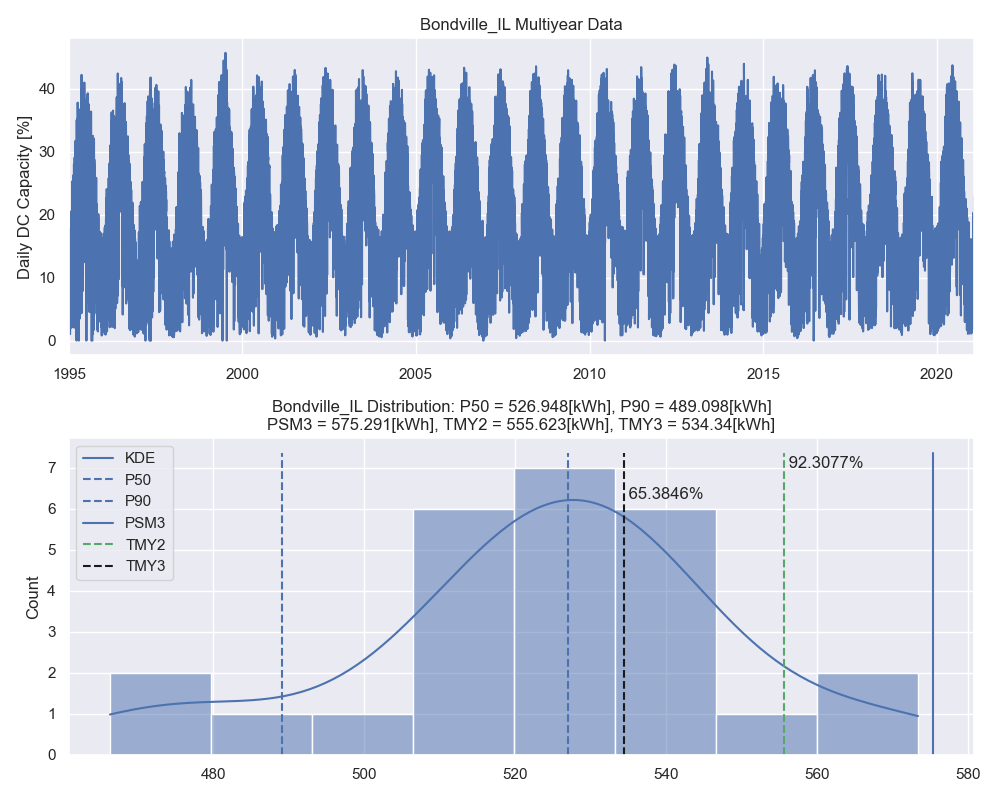
\includegraphics[width=9cm]{Bondville_IL.png}}
\caption{Daily capacity factor relative to DC nameplate for Bondville, IL, SURFRAD site (top) and distribution of annual DC energy per module (bottom).}
\label{fig:Bondville-IL}
\end{figure}

\begin{figure}[htbp]
\centerline{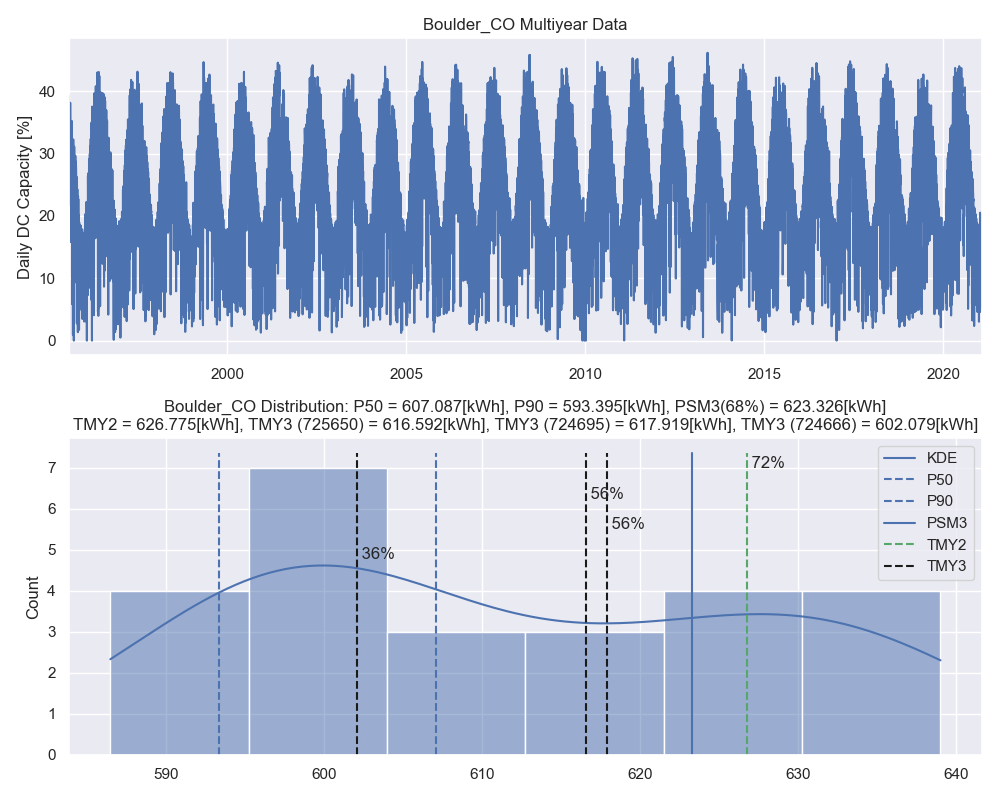
\includegraphics[width=9cm]{Boulder_CO.png}}
\caption{Daily capacity factor relative to DC nameplate for Boulder, CO, SURFRAD site (top) and distribution of annual DC energy per module (bottom).}
\label{fig:Boulder-CO}
\end{figure}

\begin{figure}[htbp]
\centerline{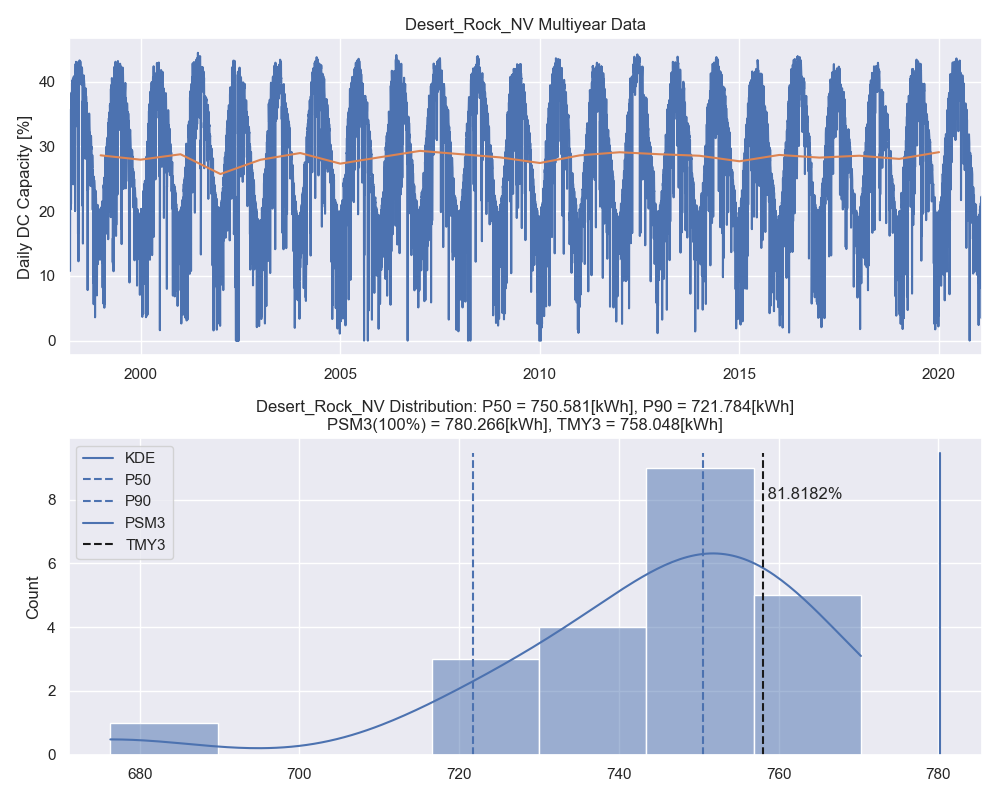
\includegraphics[width=9cm]{Desert_Rock_NV}}
\caption{Daily capacity factor relative to DC nameplate for Desert Rock, NV, SURFRAD site (top) and distribution of annual DC energy per module (bottom).}
\label{fig:Desert-Rock-NV}
\end{figure}

\begin{figure}[htbp]
\centerline{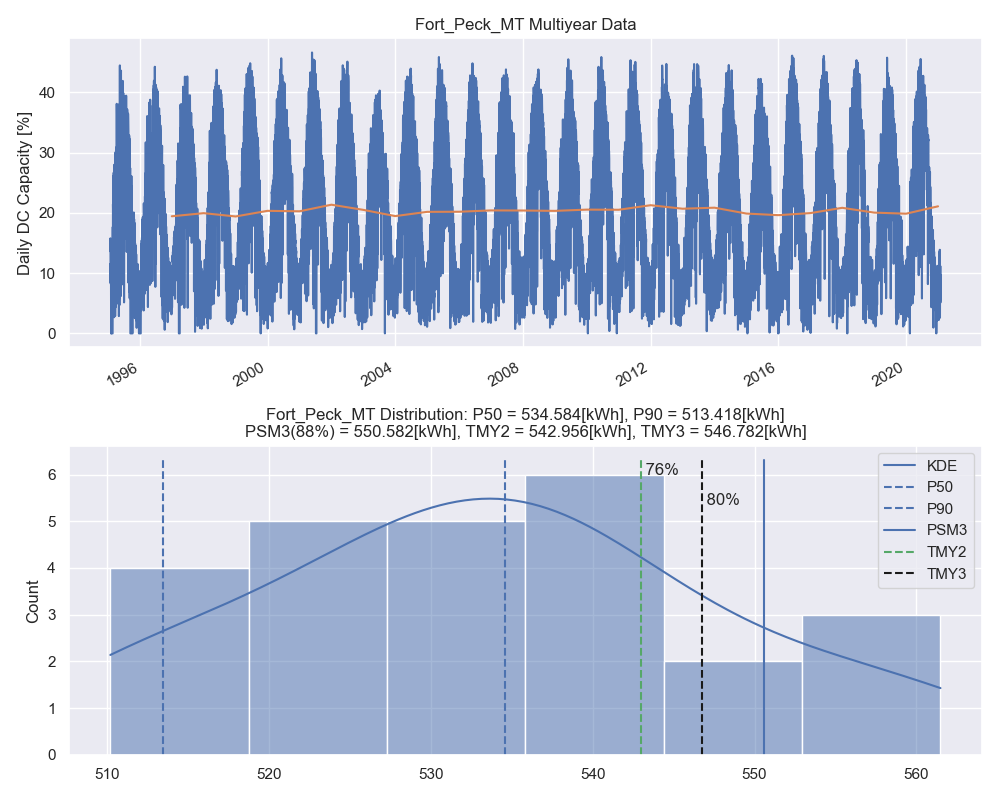
\includegraphics[width=9cm]{Fort_Peck_MT.png}}
\caption{Daily capacity factor relative to DC nameplate for Fort Peck, MT, SURFRAD site (top) and distribution of annual DC energy per module (bottom).}
\label{fig:Fort-Peck-MT}
\end{figure}

\begin{figure}[htbp]
\centerline{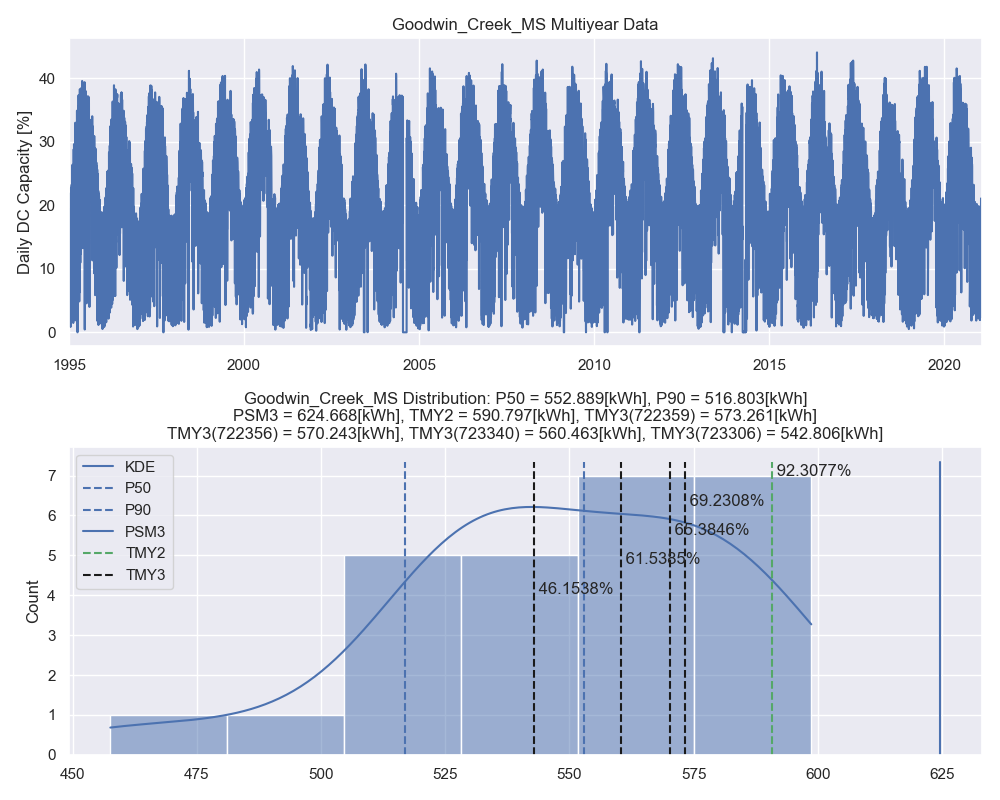
\includegraphics[width=9cm]{Goodwin_Creek_MS.png}}
\caption{Daily capacity factor relative to DC nameplate for Goodwin Creek, MS, SURFRAD site (top) and distribution of annual DC energy per module (bottom).}
\label{fig:Goodwin-Creek-MS}
\end{figure}

\begin{figure}[htbp]
\centerline{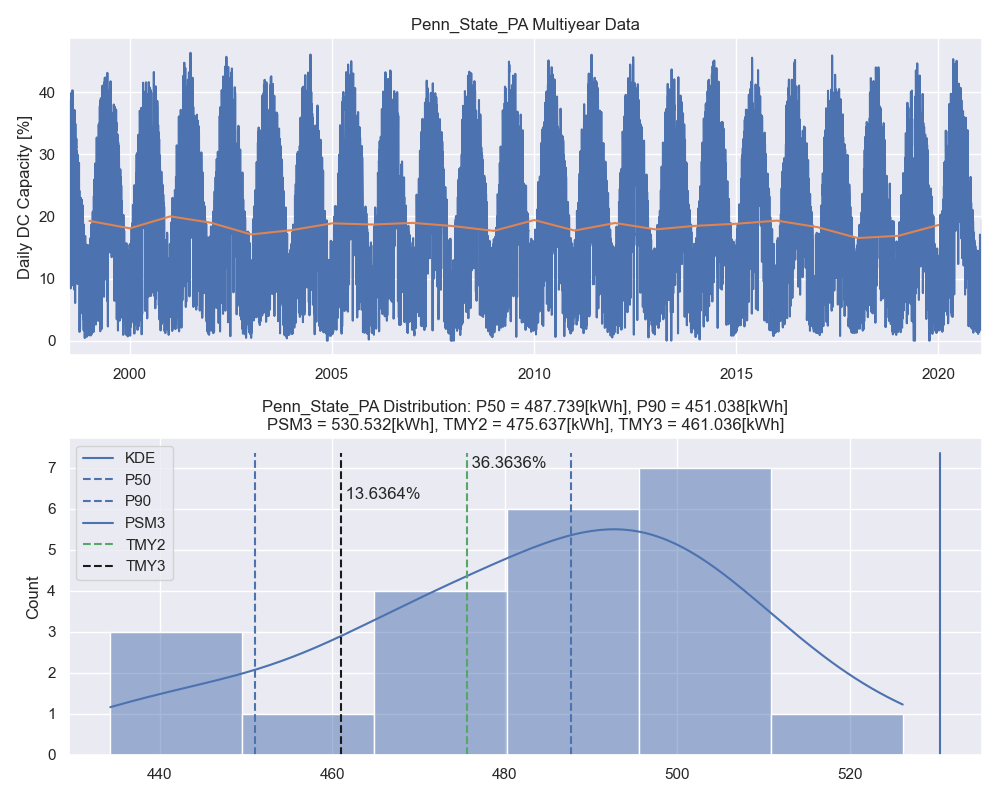
\includegraphics[width=9cm]{Penn_State_PA.png}}
\caption{Daily capacity factor relative to DC nameplate for Penn State, PA, SURFRAD site (top) and distribution of annual DC energy per module (bottom).}
\label{fig:Penn-State-PA}
\end{figure}

\begin{figure}[htbp]
\centerline{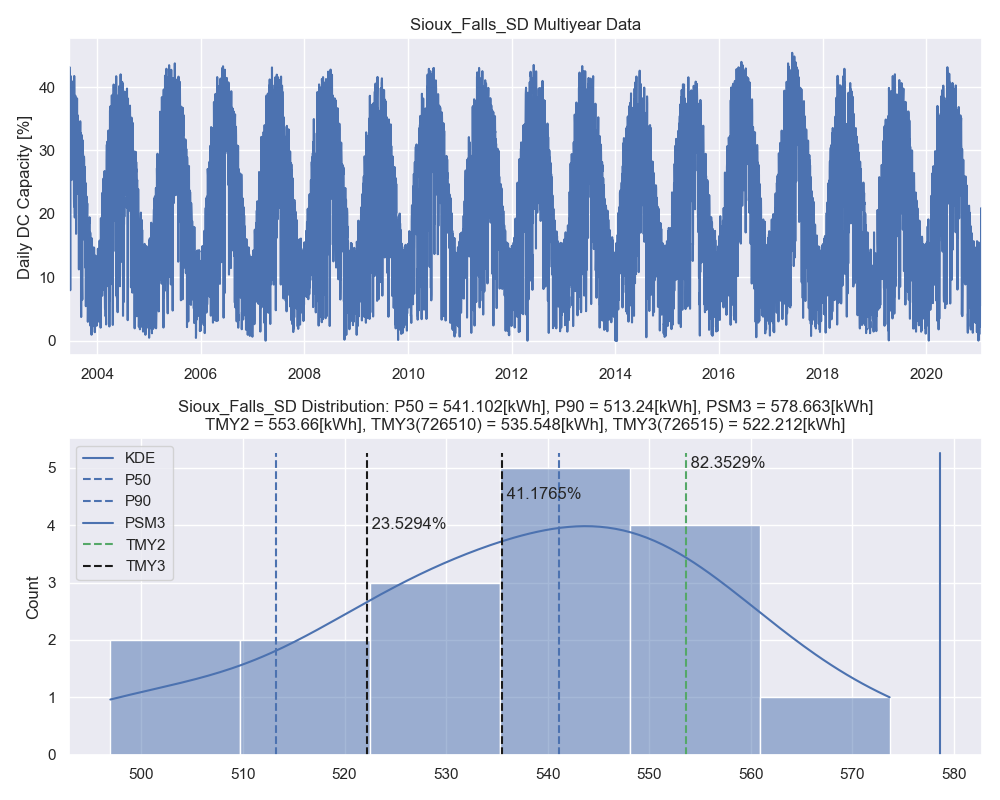
\includegraphics[width=9cm]{Sioux_Falls_SD.png}}
\caption{Daily capacity factor relative to DC nameplate for Sioux Falls, SD, SURFRAD site (top) and distribution of annual DC energy per module (bottom).}
\label{fig:Sioux-Falls-SD}
\end{figure}

\begin{table}[htbp]
\caption{Summary of Predicted SURFRAD Medians Compared with TMY}
\begin{center}
\begin{tabular}{|c|c|c|c|c|}
\hline
\textbf{SURFRAD Station} & \textbf{\textit{P50}}& \textbf{\textit{PSM3}}& \textbf{\textit{TMY2}}& \textbf{\textit{TMY3}} \\
\hline
Bondville, IL    & 20.1\%& 21.9\%& 21.1\%& 20.3\% \\
Boulder, CO      & 23.1\%& 23.7\%& 23.8\%& 23.5\% \\
Desert Rock, NV  & 28.3\%& 29.6\%&       & 28.7\% \\
Fort Peck, MT    & 20.2\%& 21.0\%& 20.7\%& 20.4\% \\
Goodwin Creek, MS& 21.0\%& 23.8\%& 22.5\%& 21.8\% \\
Penn State, PA   & 18.5\%& 20.1\%& 18.1\%& 17.4\% \\
Sioux Falls, SD  & 20.6\%& 22.0\%& 21.1\%& 20.4\% \\
\hline
\end{tabular}
\label{table:surfrad-tmy-summary}
\end{center}
\end{table}

Table~\ref{table:surfrad-tmy-summary} summarizes the results as annual capacity factors (\ref{eq:annual-capacity-factor}).

\section{Conclusions}
We studied the question of whether TMY data-sets are representative of the median predicted PV performance by comparing PV system simulations using TMY data with simulations using over 20 years of high-frequency, accurate, ground based SURFRAD measurements at 7 sites across the United States. We found that the TMY data-sets all over-predicted the median SURFRAD annual performance at 5 of 7 sites. The PSM3 predictions were greater than the median for all sites, and greater than 100\% of years in 5 of 7 sites. TMY2 predictions were greater than 70-90\% of years at 5 of 7 sites except Penn State, PA, where it was the closest to the median. Otherwise TMY3 predictions were closes to the SURFRAD median year at 5 of 7 sites, except Penn State, PA, and Desert Rock, NV, which didn't have a TMY2 site to compare with. This preliminary study suggests there is a strong positive bias for TMY2 and PSM3 but more study is necessary. In the final report, we will revise the air temperatures used in the SURFRAD simulations, which may tend to make over-predictions even greater. We will also use consistent albedo for all sites.

\bibliographystyle{IEEEtran}
% argument is your BibTeX string definitions and bibliography database(s)
\bibliography{IEEEabrv,bibliography}

\end{document}
